% DOC SETTINGS ===================================
\documentclass{article}
\usepackage[utf8]{inputenc}
\usepackage{fancyhdr}
\pagestyle{fancy}
\usepackage{geometry}
 \geometry{
 a4paper,
 total={170mm,257mm},
 left=20mm,
 top=25mm,
 }
\fancyheadoffset{0mm}
\lhead{ECE3544 HW1}
\rhead{Kavin Thirukonda 2021}
\usepackage{steinmetz}
\usepackage{listings}
\usepackage{circuitikz}
\usepackage{mathtools}  
\mathtoolsset{showonlyrefs} 
\cfoot{}
% DOC SETTINGS ===================================
\begin{document}
\section*{Problem 1 (20 points)}
The circuit shown in the diagram below is a type of CMOS AND-OR-INVERT gate. Determine the logic function that it implements. Your solution should justify your answer.
\begin{itemize}
    \item You  could  include  a  function  table  where  you show  the  status  of  each  transistor  (ON  or  OFF)  for  all possible  combinations  of  the  gate  inputs  and use  that  information to determine  the  logic  level of  the output.
    \item Instead of showing a function table, you could provide an explanation of the logic that you used to derive the logic expression from the CMOS gate schematic. This explanation should follow from the CMOS gate principles that you learned in class and that are summarized on the cover page for this assignment.
\end{itemize}
\begin{center}
    \boxed{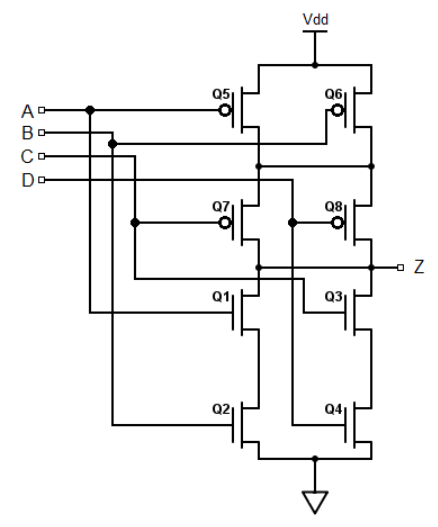
\includegraphics[width=.5\textwidth]{p1.png}}
\end{center}
\begin{center}
    if (Q1 AND Q2) OR (Q3 AND Q4) are ON, Z is 0
    
    if (Q5 OR Q6) AND (Q7 OR Q8) are ON, Z is 1
    
    \vspace{3mm}
    
    \begin{tabular}{c|c|c|c|c|c|c|c|c|c|c|c|c}
        A & B & C & D & $Q_1^N$ & $Q_2^N$ & $Q_3^N$ & $Q_4^N$ & $Q_5^P$ & $Q_6^P$ & $Q_7^P$ & $Q_8^P$ & Z\\ 
        \hline
         0 & 0 & 0 & 0 & OFF & OFF & OFF & OFF & ON  & ON  & ON  & ON  & 1\\
         0 & 0 & 0 & 1 & OFF & OFF & OFF & ON  & ON  & ON  & ON  & OFF & 1\\
         0 & 0 & 1 & 0 & OFF & OFF & ON  & OFF & ON  & ON  & OFF & ON  & 1\\
         0 & 0 & 1 & 1 & OFF & OFF & ON  & ON  & ON  & ON  & OFF & OFF & 0\\
         0 & 1 & 0 & 0 & OFF & ON  & OFF & OFF & ON  & OFF & ON  & ON  & 1\\
         0 & 1 & 0 & 1 & OFF & ON  & OFF & ON  & ON  & OFF & ON  & OFF & 1\\
         0 & 1 & 1 & 0 & OFF & ON  & ON  & OFF & ON  & OFF & OFF & ON  & 1\\
         0 & 1 & 1 & 1 & OFF & ON  & ON  & ON  & ON  & OFF & OFF & OFF & 0\\
         1 & 0 & 0 & 0 & ON  & OFF & OFF & OFF & OFF & ON  & ON  & ON  & 1\\
         1 & 0 & 0 & 1 & ON  & OFF & OFF & ON  & OFF & ON  & ON  & OFF & 1\\
         1 & 0 & 1 & 0 & ON  & OFF & ON  & OFF & OFF & ON  & OFF & ON  & 1\\
         1 & 0 & 1 & 1 & ON  & OFF & ON  & ON  & OFF & ON  & OFF & OFF & 0\\
         1 & 1 & 0 & 0 & ON  & ON  & OFF & OFF & OFF & OFF & ON  & ON  & 0\\ 
         1 & 1 & 0 & 1 & ON  & ON  & OFF & ON  & OFF & OFF & ON  & OFF & 0\\
         1 & 1 & 1 & 0 & ON  & ON  & ON  & OFF & OFF & OFF & OFF & ON  & 0\\
         1 & 1 & 1 & 1 & ON  & ON  & ON  & ON  & OFF & OFF & OFF & OFF & 0\\
    \end{tabular}
    
    \vspace{2mm}
    
    The simplest form of the Boolean equation this represents is \boxed{Z = A'C' + B'C' + A'D' + B'D'} 
\end{center}
\newpage
\section*{Problem 2 (20 points)}
The circuit shown in the diagram below is a type of CMOS OR-AND-INVERT gate. Determine the logic  function  that  it  implements.  Your  solution  should  justify  your  answer.  Follow  the  guidance  given  in Problem 1.

\begin{center}
    \boxed{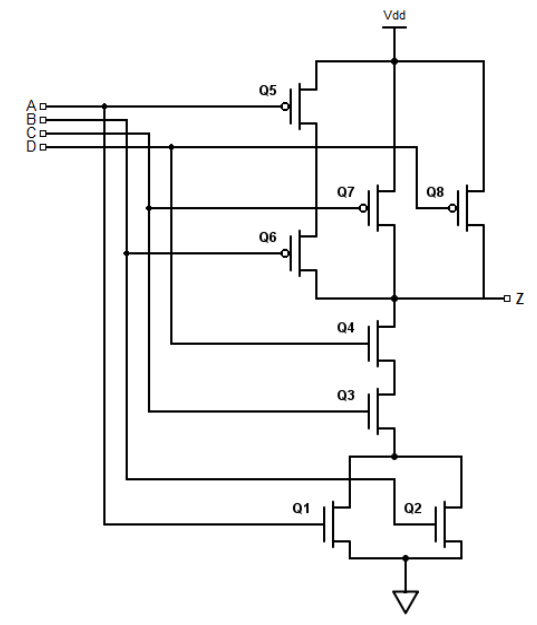
\includegraphics[width=.5\textwidth]{p2.png}}
\end{center}
\begin{center}
    if (Q1 OR Q2) AND (Q3 AND Q4) are ON, Z is 0
    
    if (Q5 AND Q6) OR Q7 OR Q8 are ON, Z is 1
    
    \vspace{3mm}
    
    \begin{tabular}{c|c|c|c|c|c|c|c|c|c|c|c|c}
        A & B & C & D & $Q_1^N$ & $Q_2^N$ & $Q_3^N$ & $Q_4^N$ & $Q_5^P$ & $Q_6^P$ & $Q_7^P$ & $Q_8^P$ & Z\\ 
        \hline
         0 & 0 & 0 & 0 & OFF & OFF & OFF & OFF & ON  & ON  & ON  & ON  & 1\\
         0 & 0 & 0 & 1 & OFF & OFF & OFF & ON  & ON  & ON  & ON  & OFF & 1\\
         0 & 0 & 1 & 0 & OFF & OFF & ON  & OFF & ON  & ON  & OFF & ON  & 1\\
         0 & 0 & 1 & 1 & OFF & OFF & ON  & ON  & ON  & ON  & OFF & OFF & 1\\
         0 & 1 & 0 & 0 & OFF & ON  & OFF & OFF & ON  & OFF & ON  & ON  & 1\\
         0 & 1 & 0 & 1 & OFF & ON  & OFF & ON  & ON  & OFF & ON  & OFF & 1\\
         0 & 1 & 1 & 0 & OFF & ON  & ON  & OFF & ON  & OFF & OFF & ON  & 1\\
         0 & 1 & 1 & 1 & OFF & ON  & ON  & ON  & ON  & OFF & OFF & OFF & 0\\
         1 & 0 & 0 & 0 & ON  & OFF & OFF & OFF & OFF & ON  & ON  & ON  & 1\\
         1 & 0 & 0 & 1 & ON  & OFF & OFF & ON  & OFF & ON  & ON  & OFF & 1\\
         1 & 0 & 1 & 0 & ON  & OFF & ON  & OFF & OFF & ON  & OFF & ON  & 1\\
         1 & 0 & 1 & 1 & ON  & OFF & ON  & ON  & OFF & ON  & OFF & OFF & 0\\
         1 & 1 & 0 & 0 & ON  & ON  & OFF & OFF & OFF & OFF & ON  & ON  & 1\\ 
         1 & 1 & 0 & 1 & ON  & ON  & OFF & ON  & OFF & OFF & ON  & OFF & 1\\
         1 & 1 & 1 & 0 & ON  & ON  & ON  & OFF & OFF & OFF & OFF & ON  & 1\\
         1 & 1 & 1 & 1 & ON  & ON  & ON  & ON  & OFF & OFF & OFF & OFF & 0\\
    \end{tabular}
    
    \vspace{2mm}
    
    The simplest form of the Boolean equation this represents is \boxed{Z = C' + D' + A'B'} 
\end{center}
\newpage
\section*{Problem 3 (30 points)}
Draw the CMOS transistor schematic for a “gate” that implements these Boolean functions. Your implementation must be transistor-efficient.
\subsection*{a)}
\begin{align}
Z_1 &= (A+ BCD)'\\
&= A' \cdot(B'+C'+D')\\
&=  A'B'+ A'C'+ A'D'
\end{align}
\begin{center}
    \boxed{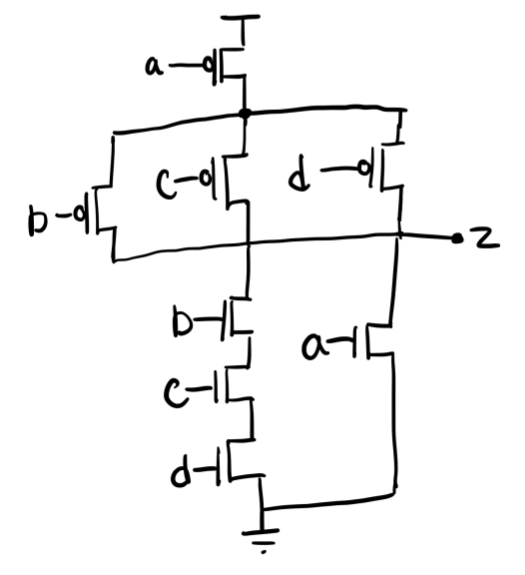
\includegraphics[width = .4\textwidth]{p3b.png}}
\end{center}
\subsection*{b)}
\begin{align}
    Z_2 &= [A \cdot (B+ C)\cdot D]'\\
    &= A' + (B + C)' + D' \\
    &= A' + B'C' + D'
\end{align}
\begin{center}
    \boxed{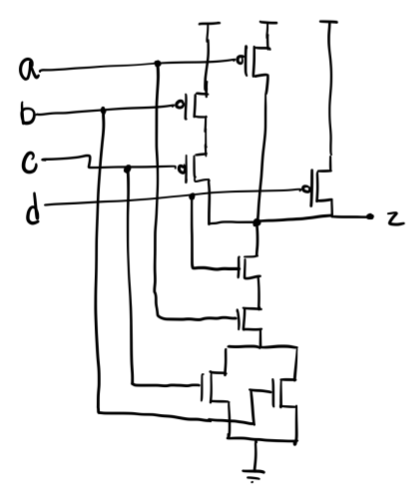
\includegraphics[width = .4\textwidth]{p3a.png}}
\end{center}
\newpage
\section*{Problem 4 (30 points)}
A particular CMOS gate operates at a particular switching frequency $f_1$, employs a particular load capacitance  $C_1$,  and  switches the  load  through a  particular  voltage  $V_1$.  It  therefore  consumes  a  calculable amount of dynamic power, which we will call P. 
\vspace{5mm}

A second CMOS gate operates at a switching frequency that is 25 percent higher than that of the first CMOS gate –that is, it has a switching frequency $f_2$ = 1.25 * $f_1$.However, the two CMOS gates consume the same amount of dynamic power.
\vspace{5mm}

Call the load capacitance of the second CMOS gate $C_2$. Call the voltage through which the second CMOS gate is switched $V_2$.

\subsection*{a)}
Suppose that $V_2$ = $V_1$. By what factor does $C_2$ relate to $C_1$?
\begin{align}
    P = C_1V_1^2f_1 = C_2V_2^2f_2\\
    \Rightarrow C_1f_1 = C_2(1.25 \cdot f_1)\\
    \Rightarrow \boxed{C_1 = C_2 \cdot 1.25}\\
\end{align}
\subsection*{b)}
Now suppose that $C_2$= $C_1$. By what factor does $V_2$ relate to $V_1$?
\begin{align}
    P = C_1V_1^2f_1 = C_2V_2^2f_2\\
    \Rightarrow V_1^2f_1 = V_2^2(1.25 \cdot f_1)\\
    \Rightarrow \sqrt{V_1^2} = \sqrt{V_2^2\cdot(1.25)}\\
    \Rightarrow \boxed{V_1 = V_2\cdot 1.118}\\
\end{align}
\newpage
\end{document}
